\chapter{aCoral内存分布}
前一章中,多次提到了aCoral最终会在0x30000000这个地址运行,也就是内存sdram所在的地址。
那为什么一定是这个地址呢?aCoral在执行copy\_self的时候,copy到0x30000001行不行?
要解释这个问题,我们要先了解两个概念:存储地址和运行时地址。

\section{存储地址和运行时地址}

存储地址也可以叫加载地址。因为我们的程序是要存储在非易失性存储器上的,比如nor flash和nand flash。
程序存储在这些存储器的地址就叫做存储地址。比如aCoral被烧写到nand flash的0地址后,它的存储地址就是从0开始的一连串地址。

运行时地址是程序运行时应该在的地址,注意是应该,表示程序最好在这个地址运行。
如果程序全部由位置无关代码构成,那即使不在运行时地址运行,程序也不会出错。但是只要有位置相关代码,程序就g了。
运行时地址表示程序人员对代码运行时的一种期待和要求。
aCoral在mini2440开发板的运行时地址为0x30000000,所以当我们把flash中的acoral整个复制到0x30000000之后的区域后,
我们就说aCoral此时已经来到了它的运行时地址。

不同的开发板,内存的地址不同,aCoral的运行时地址就会不同。mini2440就是0x30000000。
那我们在哪里指定这个地址呢?这就是链接脚本做的事了。当然链接脚本不仅指定了运行时地址,还决定了整个aCoral镜像的结构,也就是aCoral被复制到sdram中之后的内存分布。
链接脚本位于
\begin{lstlisting}
 hal\s3c2440\acoral.lds
\end{lstlisting}

\section{aCoral链接脚本}

链接脚本是给链接器看的。链接器会按照链接脚本定义的规则,把aCoral源码中编译出来的一个个可重定位文件(.o)进行链接,最终得到acoral.bin。
链接脚本内容如下:

\begin{lstlisting}
ENTRY(__ENTRY)

MEMORY
{  
	    ram (wx)  : org = 0x030000000,   len = 64M
}
SECTIONS
{
	.text : 
	{
		text_start = .;
	       	* (.text)
     		* (.init.text)
		* (.rodata*)
	}>ram 
	
	.data ALIGN(4):
	{  
		*(.acoral1.call) 
		*(.acoral2.call) 
		*(.acoral3.call) 
		*(.acoral4.call) 
		*(.acoral5.call) 
		*(.acoral6.call) 
		*(.acoral7.call) 
		*(.acoral8.call) 
		*(.acoral9.call) 
		*(.acoral10.call) 
	     	*(.data)
		*(.data.rel)
		*(.got)
		*(.got.plt)
	} >ram
	
	.bss ALIGN(4): 
	{ 
		bss_start = .;    
		* (.bss)
     		. = ALIGN(4) ;
	} >ram
	bss_end = .;    

	stack_base = 0x33ffff00;
	MMU_base   =   0x33f00000;

	SYS_stack_size   =  0x200;      
	SVC_stack_size   =  0x200;    
	Undef_stack_size =  0x100;        
	Abort_stack_size =  0x100;     
	IRQ_stack_size   =  0x200;       
	FIQ_stack_size   =  0x0;   

	FIQ_stack        =  stack_base; 
	IRQ_stack        =  FIQ_stack   - FIQ_stack_size;  
	ABT_stack        =  IRQ_stack   - IRQ_stack_size;  
	UDF_stack        =  ABT_stack   - Abort_stack_size;    
	SVC_stack        =  UDF_stack   - Undef_stack_size;    
	SYS_stack        =  SVC_stack   - SVC_stack_size;  
	heap_start = (bss_end + 3)&( ~ 3);  
	heap_end = MMU_base - 0x1000;
}  

\end{lstlisting}

ENTRY关键字定义了整个源码的入口就是标号\_ENTRY。这个标号定义在
\begin{lstlisting}
 hal\s3c2440\src\start.S
\end{lstlisting}

所以start.S中\_ENTRY标号处的
\begin{lstlisting}
 b	ResetHandler
\end{lstlisting}

就是aCoral上电后执行的第一行代码。

MEMORY关键字将目标开发板的内存sdram分块,这里只分为一块区域,名为ram,起始地址就是0x30000000。

SECTIONS关键字中,镜像文件将被分段,包括我们通常说的代码段.text,数据段.data,未定义数据段.bss等。
.text段的最后使用“>ram”指定了.text段将被放在内存的ram区域,也就是说代码段理论上应该在0x30000000的地址开始运行,这就是运行时地址的由来。
之后的数据段和bss段也都是放在ram这个内存区域,紧接着代码段放置。

之后还定义了arm各个模式的栈空间,最后定义了heap堆的地址空间。
这里heap堆的起始地址heap\_start和终止地址heap\_end,其实就是aCoral可用的内存空间,大小大概是64M不到一点。
aCoral下载到内存后的整个内存分布的具体细节如图\ref{aCoral内存分布}所示。

\begin{figure}[H]
	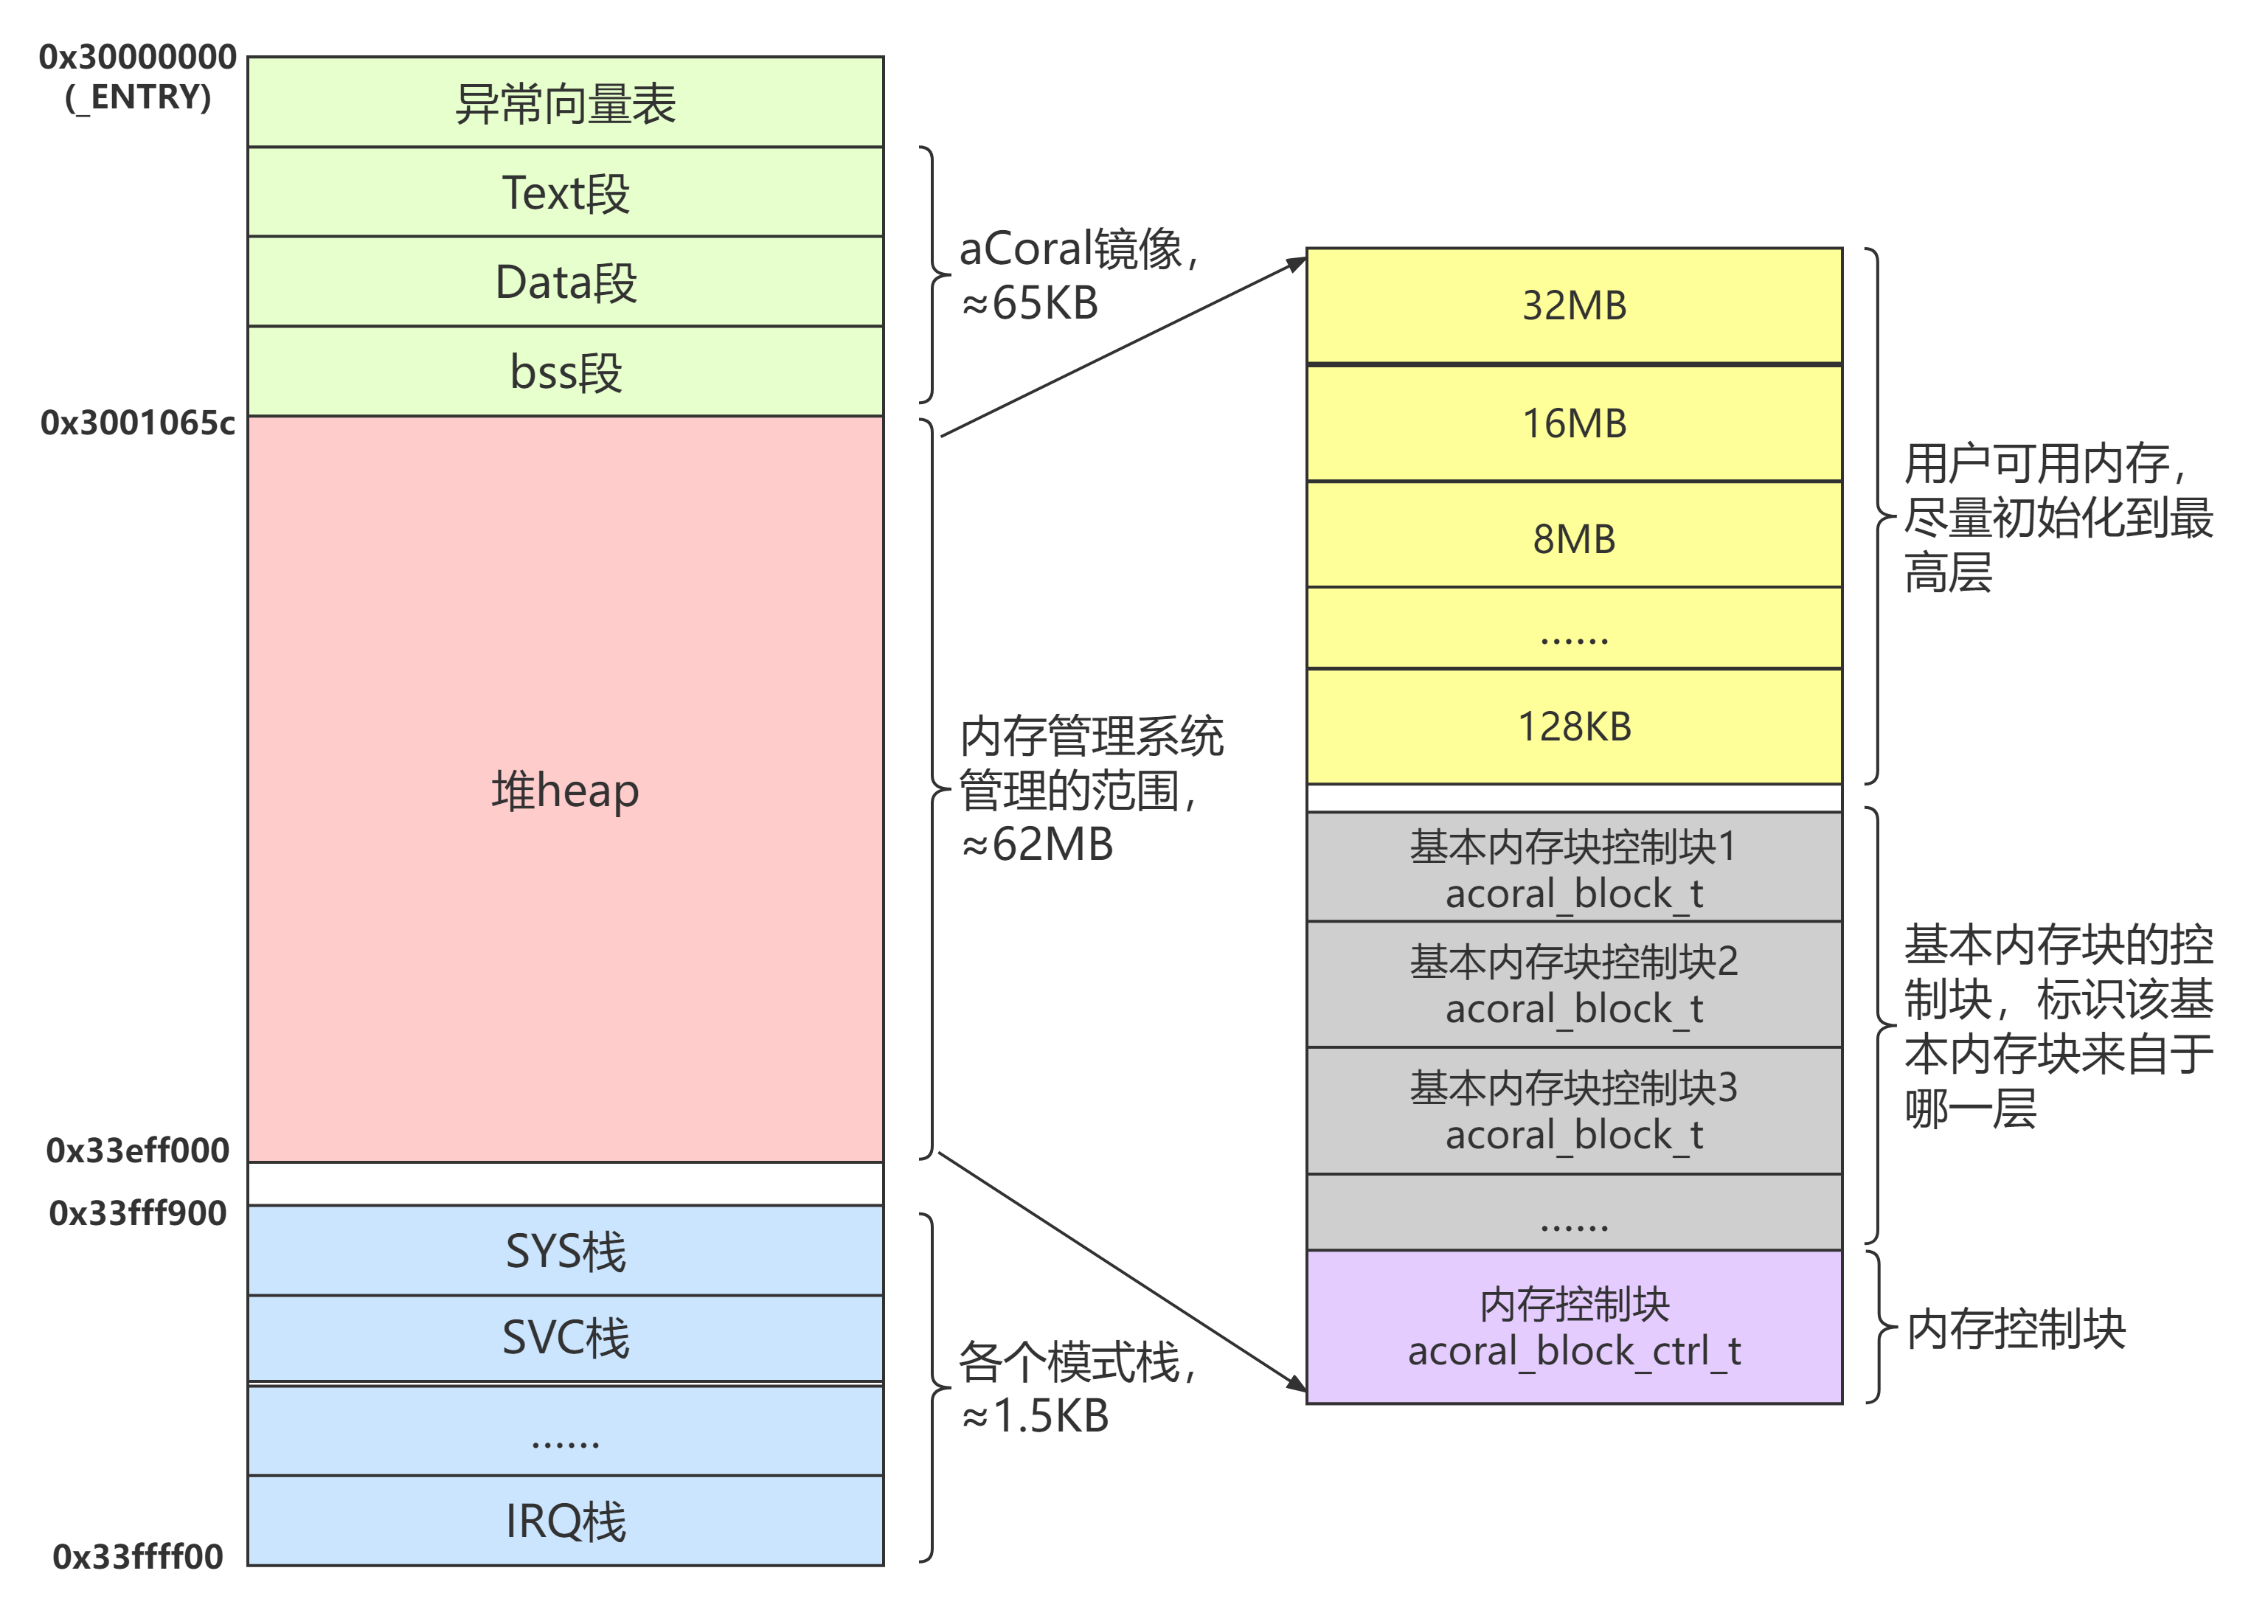
\includegraphics[width=0.9\textwidth]{aCoral内存分布.png}
	\caption{aCoral内存分布}
	\label{aCoral内存分布}
\end{figure}


